\section{Mission A}
\subsection{Sous-Mission A1}

	\begin{vwcol}[widths={0.65,0.2}, rule=0pt]
		\begin{minipage}{0.7\textwidth}
			\paragraph{Objectifs de la mission}

			Determiner l'emplacement la plus élevé sur l'image en se basant sur le pixel le plus clair. Cet emplacement servira plus tard à l'atterissage d'une mission interplanetaire. On doit donc déterminer les coordonnées du pixel le plus clair de l'image.
		\end{minipage}

		\begin{minipage}{0.3\textwidth}
			\begin{flushright}
				\paragraph{Technique utilisée}
			
				Analyse pixel à pixel
			\end{flushright}
		\end{minipage}
	\end{vwcol} 

	\begin{figure}[h]
		\centering
		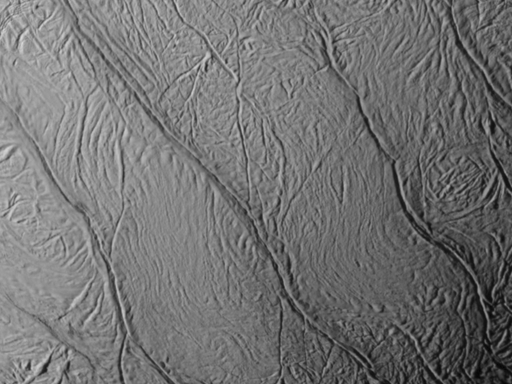
\includegraphics[scale=0.6]{images/Encelade_surface.png}
	\end{figure}
	\vspace{-0.3cm}

	\paragraph{Procédé}	Apres avoir déterminé la couleur la plus claire de l'image avec la fonction \emph{\texttt{max()}}, nous avons parcouru chacun des pixels pour retenir les coordonnées de la couleur la plus claire. On recupère alors une matrice contenant les coordonnées de tous les pixels les plus clairs. Dans le cas de cette mission, un seul pixel permet l'atterissage, il se situe aux coordonnées $x=22$ et $y=38$.